


\subsection{Representación}

La forma estándar de representar un polígono es simplemente enumerar los vértices del polígono
en sentido horario o antihorario. Pero los vértices como se representa ?. Un vértice nos es mas que un punto en este caso en la plano 2D por tanto se va definir con una valor en la coordenada X y otro valor en la coordenada Y.

Por tanto para representar un polígono primero necesitamos representar un vértice y luego con una colección de vertices podemos representar computacional un polígono.

\subsection{Perímetro}

El perímetro de un polígono (ya sea convexo o cóncavo) con $n$ vértices dados en algún orden
(ya sea en el sentido de las agujas del reloj o en el sentido contrario a las agujas del reloj) se puede calcular a través de la suma de las distancias euclidianas entre todos los pares consecutivos de vértices del polígono.

\subsection{Área}

Esto es fácil de hacer si pasamos por todos los lados y agregamos áreas trapezoidales limitadas por cada lado y el eje x. El área debe tomarse con señal para que se reduzca el área adicional. Por lo tanto, la fórmula es la siguiente:


$$ A = \sum_{(p,q)\in \text{lados}} \frac{(p_x - q_x) \cdot (p_y + q_y)}{2} $$



Otra variante es elegir un punto $O$ arbitrariamente, iterar sobre todos los bordes agregando el área orientada del triángulo formado por el borde y el punto $O$. Nuevamente, debido al signo de área, se reducirá el área extra. Este método es mejor ya que puede generalizarse a casos más complejos (como cuando algunos lados son arcos en lugar de líneas rectas).

%$$ A = \frac{1}{2} \times \begin{bmatrix}
% x_{0}	& y_{0} \\
% x_{1}	& y_{1} \\
% x_{2}	& y_{2} \\
% \dots	& \dots  \\
%x_{n-1}	& y_{n-1}
%\end{bmatrix} = \frac{1}{2} \times (x_{0} \times y_{1} +x_{1} \times y_{2} + \dots +x_{n-1} \times y_{0} - x_{1} \times y_{0} - x_{2}  \times y_{1} - \dots - x_{0} \times y_{n-1}) $$

\subsection{Comprobar si es convexo}

Se dice que un polígono es convexo si cualquier segmento de línea dibujado dentro del polígono no
intersecar cualquier lado del polígono. De lo contrario, el polígono se llama cóncavo. En la figura de abajo a la izquierda tenemos un polígono convexo mientras a la derecha tenemos un polígono cóncavo

\begin{figure}[h!]
	\centering
	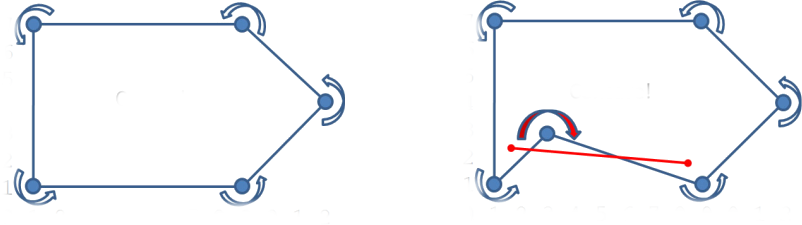
\includegraphics[width=0.7\linewidth]{img/poligono_convexo_concavo}
	\caption{}
	\label{fig:poligonoconvexoconcavo}
\end{figure}

Sin embargo, para probar si un polígono es convexo, existe un enfoque computacional más sencillo que
"tratando de verificar si todos los segmentos de línea se pueden dibujar dentro del polígono". Simplemente podemos comprobar si los tres vértices consecutivos del polígono forman los mismos giros (todos los giros a la izquierda/CCW si los vértices se enumeran en el sentido contrario a las agujas del reloj o todos giran a la derecha/cw si los vértices están enumerados en el sentido de las agujas del reloj). Si podemos encontrar al menos un triple donde esto es falso, entonces el polígono es cóncavo. Es importante notar que los puntos que conforman el polígono nunca debe existir tres vértices consecutivos que sean colineales entre sí.


\subsection{Posición de un punto con respecto a un polígono}

Otra prueba común que se realiza en un polígono $P$ es verificar si un punto $pt$ está dentro o fuera
polígono $P$. En la imagen se reflejan tres situaciones del problema planteado en las dos primeras el punto esta dentro mientras en el tercer caso esta fuera.

% TODO: \usepackage{graphicx} required
\begin{figure}[h!]
	\centering
	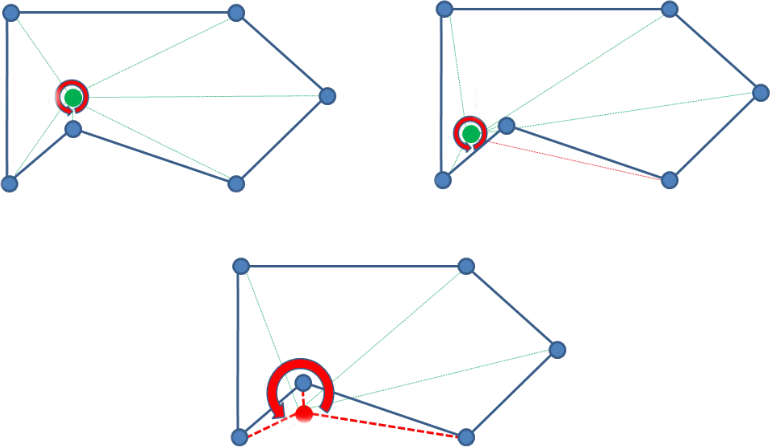
\includegraphics[width=0.6\linewidth]{img/poligono_convexo_punto}
	\label{fig:poligonoconvexopunto}
\end{figure}


El procedimiento es calculando las sumas de los ángulos entre tres puntos de todas las posibles tripletas de la forma {P[i],pt,P[i+1]} donde (P[i]-P[i+1]) son lados consecutivos del polígono $P$ , cuidando los giros a la izquierda (sumar el ángulo) y los giros a la derecha (restar el ángulo) respectivamente. Si la suma final es $2\pi$ (360 grados), entonces $pt$ está dentro del polígono $P$. La otro posición que puede tomar un punto con respecto a un polígono es que este sobre un lado del polígono en este caso va depender de lo que plantee el problema para este caso, en la mayoría de los casos se considera dentro. Para su comprobación basta con cada posible  tripleta {P[i],pt,P[i+1]} comprobar si con colineales si al menos uno cumple el punto está en el borde del polígono.